\chapter{Experimental Evaluation}
\label{experimental_evaluation}
\thispagestyle{empty}

\begin{quotation}
{\footnotesize
\noindent \emph{It doesn't matter how beautiful your theory is, it doesn't matter how smart you are, if it doesn't agree with experiment, it's wrong.}
\begin{flushright}
R.P. Feynman
\end{flushright}
}
\end{quotation}
\vspace{0.5cm}

\noindent In the previous chapter we presented the REMPS algorithm, able to optimize the model and the policy in the context of discretes and continuous CMDPs. In this chapter we perform an experimental evaluation of REMPS. In \cref{sec:chain} we consider the chain environment, that is a toy problem for which we can visualize the return surface and we can easily understand the behaviour of our algorithm.
In \cref{sec:cartpole} we evaluate the performance of our algorithm on the discrete-actions, continuous-states, cart-pole problem, a standard RL benchmark. We compare REMPS with the G(PO)MDP \citep{gpomdp} extension for CMDPs (see \cref{gpomdp_cmdp}).
In \cref{sec:torcs} we consider an autonomous driving and configuration problem in a complex environment: TORCS. The goal of the TORCS experiment is to show the benefit of environment configuration in a complex task, similar to real world tasks.
\section{Chain Problem} \label{sec:chain}

\begin{figure}
\centering
	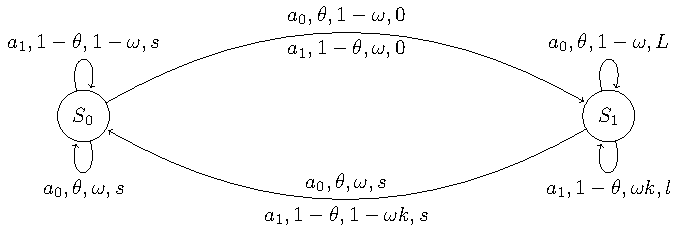
\includegraphics[width=\textwidth]{pictures/chain}
	\caption{Chain problem. On the edges we have (action, action probability, transition probability, reward).}
	\label{fig:chain}
\end{figure}

We use the chain problem as a proof of concept to show the benefits of our algorithm. Using this environment we experimentally validate the ability of REMPS to overcome local minima in the return landscape. \newline The environment in illustrated in \cref{fig:chain}. There are two actions available to the agent denoted with $a_0$ and $a_1$. The policy is very simple and has only one parameter:
\begin{align}
	\pi_\theta(a_0 | s) &=  \theta \; \forall s \in \mathcal{S}, \\
	\pi_\theta(a_1 | s) &=  1 - \theta \; \forall s \in \mathcal{S} \, .
\end{align}
Thus the policy is uniquely defined by the parameter $\theta \in [0,1]$, that is the probability of selecting action $a_0$ and it is the same on all states.
The model has only one parameter, $\omega$, that is the probability of action failure.
Action $a_0$ (forward), if successful, brings the agent to state $s_1$. Action $a_1$ (backward), if successful, brings the agent to state $s_0$.
The agent gets an high reward, $L > 0$, if, starting from state $s_1$ executes successfully action $a_0$. The agent gets a smaller reward $l $, ($0 < l < L$) if it lands in state $s_1$ starting from $s_1$ but executing action $a_1$. Agent gets an even smaller reward, $s$ ($0 < s < l$) when it lands in state $s_0$. The parameter $k$ is not configurable and it has been added to avoid symmetries in the return surface. In the chain problem we are in the ideal case, the model is known, thus we can project the stationary distribution directly.
We initialized the model parameters to $\omega_0$ and the policy parameter to $\theta_0$ such that the initial position in the return landscape is near a local minima. Starting from this position a gradient method should point toward the local maxima, while we empirically demonstrate the ability of our algorithm to reach the pair ($P^*$,$\pi^*$) yielding maximum performance in this environment. The average reward surface as function of the model and policy parameters is illustrated in \cref{fig:chain-rew}. \newline
\begin{figure}[!tb]
\centering
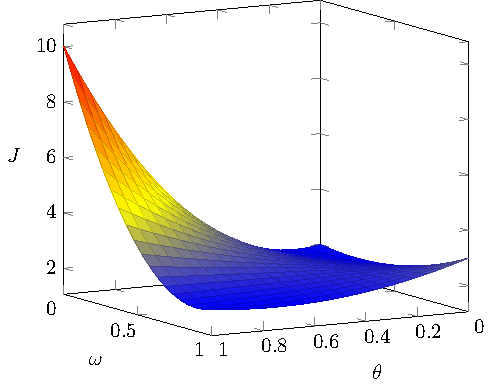
\includegraphics[width=0.8\textwidth]{plots/chain/plot_chain_surface}
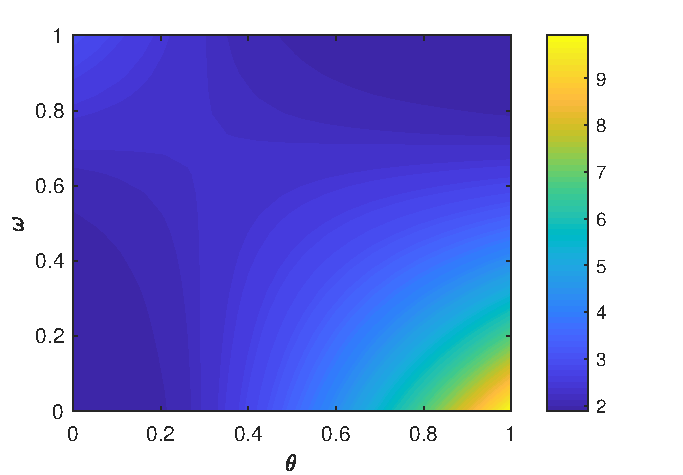
\includegraphics[width=0.8\textwidth]{plots/chain/plot_chain_colormap}
	\caption{Different representations of the average reward surface of the chain experiment as function of model and policy parameters. There is a local maximum in $\theta=0, \omega=1$, a global maximum in $\theta=1, \omega=0$. We start our algorithm near the local minima in $\theta=0.33, \omega=0.66$.}
	\label{fig:chain-rew}
\end{figure}
Table \ref{tab:chain-hyperparameters} summarizes the parameters used in our experiments. \newline
\begin{table}[t]
\centering
\begin{tabular}{ c c}
  \toprule			
  Parameter & Value \\
  \midrule
  $k$ & $0.2$ \\
  $L$ & $10$ \\
  $l$ & $8$ \\
  $s$ & $2$ \\
  $\omega_0$ & $0.8$ \\
  $\theta_0$ & $0.2$ \\
  num of samples & $2 \cdot 10^4$ \\
  num of steps per episode & $5 \cdot 10^2$ \\
\bottomrule
\end{tabular}
\caption{Hyper-parameters used in our chain experiments.} \label{tab:chain-hyperparameters}
\end{table}
We compare the result of our algorithm with G(PO)MDP over model and policy parameters.
It is possible to see that G(PO)MDP, being a gradient method follows the slope of the objective function and it is attracted by the \textit{local} maximum in $\theta=0, \omega=1$. REMPS outperforms G(PO)MDP reaching the \textit{global} maximum in $\theta=1, \omega=0$ after few iterations. We perform different runs varying the $\epsilon$ parameter to show the effect of the parameter. Results are shown in \cref{fig:chain-exp}.

\begin{figure}[!tb]
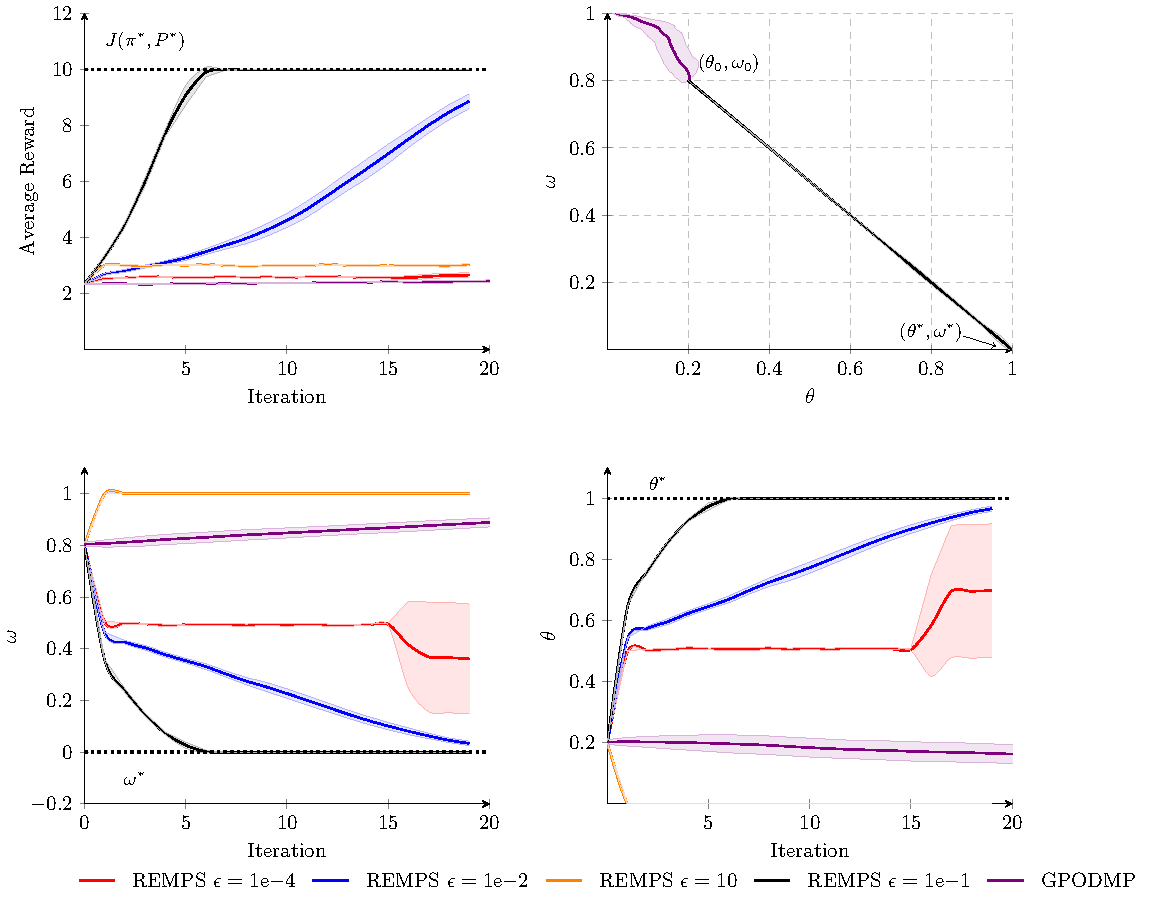
\includegraphics[width=1\textwidth]{plots/chain/plot_chain_all}
\caption{Chain experiment. Top left: average reward of REMPS and GPOMDP. Top right: updates of the model and policy parameter of  GPOMDP and REMPS. Bottom left: shows the updates of the model parameter $\omega$. Bottom right: updates of the policy parameter $\theta$. Shaded areas represent the $95\%$ confidence interval over 10 runs of the algorithm.}
\label{fig:chain-exp}
\end{figure}  

\subsection{Sensitivity to $\epsilon$}
The choice of $\epsilon$ is critical and problem-dependent. A too small $\epsilon$ causes a premature convergence of REMPS to local maximum. A too high $\epsilon$ yields imprecise estimation of the performance of the model-policy target and causes an imprecise projection on the space of possible probability distributions. \cref{fig:jeps} shows the performance of the best model-policy found as function of $\epsilon$. 
We show the value of the primal that is the value of the objective function without any constraint on the policy and model. We can see that the value of the primal is greater than the actual value of the objective after the projection, thus the projection yields a degradation of the performance. The performance degradation is due to the following reason. Moving too far away from the current stationary distribution the primal solution might not be representable using our hypothesis space. Performing a Moment Projection we obtain a  a performance degradation with respect to the original solution.
\begin{figure}[!tb]
\centering
	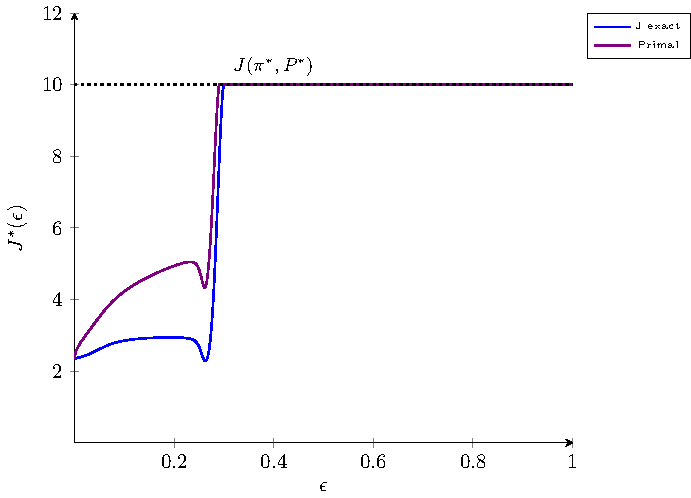
\includegraphics[width=1\textwidth]{plots/chain/plot_j_epsilon}
	\caption{Average reward and primal of the best model-policy couple in the chain experiment as function of $\epsilon$ using the projection of the discounted stationary state distribution.}
	\label{fig:jeps}
\end{figure}
\subsection{Sensitivity to parameter initialization}
REMPS behaves consistently with respect to a random initialization of model and policy parameters. In \cref{fig:chain-random-init} we can see that REMPS updates the model and policy parameters toward the global maximum while GPOMDP updates vary with the initial parameters. In the GPOMDP learning curve it is possible to see clearly the two attractors. REMPS shows a stable behaviour in the case of few model parameters and complex return landscape. 
\begin{figure}[!tb]
\centering
	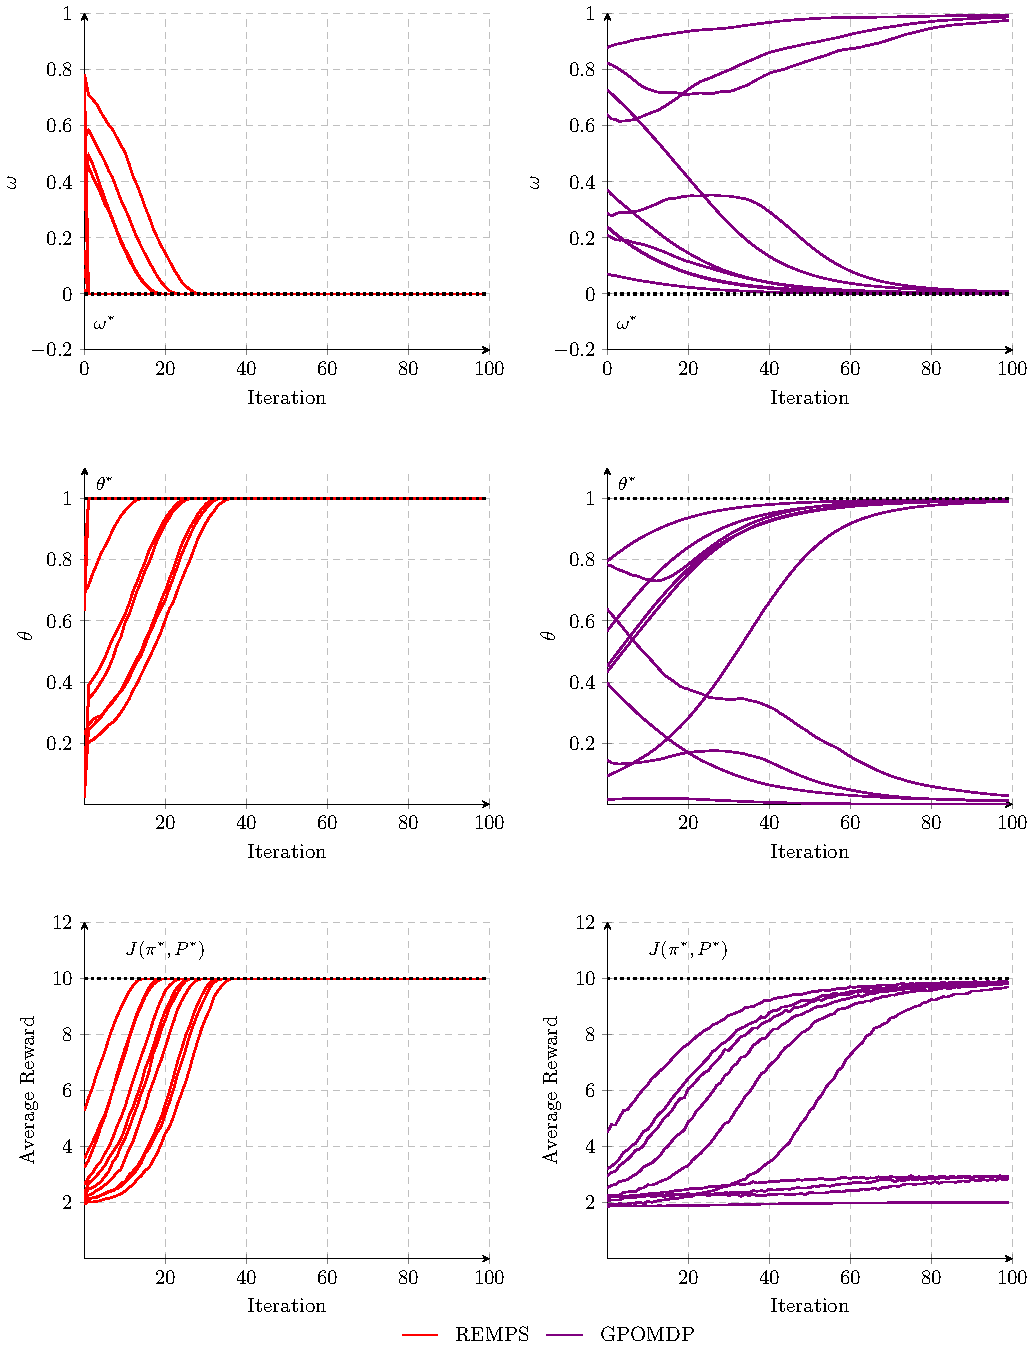
\includegraphics[width=1\textwidth]{plots/chain/plot_random_init}
	\caption{Chain experiment with random initialization of model and policy parameter. Comparison between GPOMDP and REMPS. Top: model parameter. Center: policy parameter. Bottom: average reward.}
	\label{fig:chain-random-init}
\end{figure}
\subsection{Comparison with SPMI}
SPMI is, at the moment of writing, the unique algorithm proposed for CMDPs. We compare in this section the comparison between SMPI and REMPS.
In \cref{fig:chain-spmi} we show the behaviour of the variants of SPMI on the chain experiment. We can easily notice that SPMI requires a huge number of iterations before convergence. While REMPS converges approximately after $10$ iterations, SPMI requires a number of iterations in the order of $10^3$. This is due to the conservative step size of safe approaches. SPMI, SPMI-alt, SPMI-sup and SPI-SMI reach the global maximum while SMI-SPI goes (very slowly) to the local maximum. SMI-SPI is not able to reach the global maximum since it alternates a model improvement step to a policy improvement step considering the two components in a separate manner. \newline
We recall that SPMI is applicable to the chain experiment since this environment has a discrete state space and a discrete action space, while the standard version of this algorithm cannot be applied to the environments presented later in this chapter.
 
\begin{figure}[!tb]
\centering
	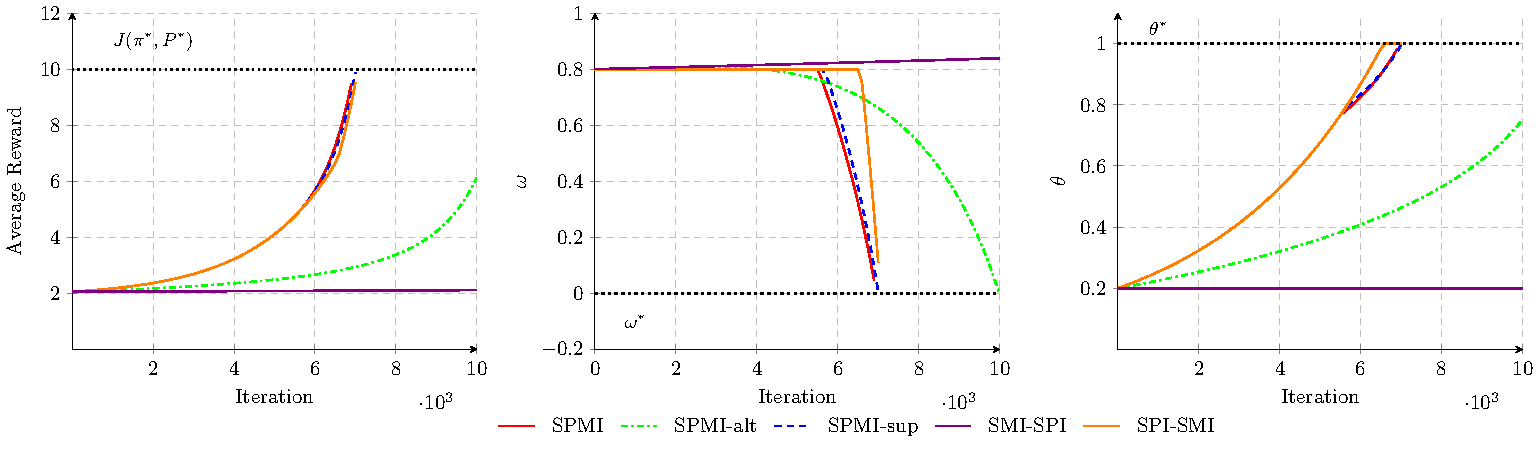
\includegraphics[width=1\textwidth]{plots/chain/plot_spmi}
	\caption{SPMI on the chain experiment. Left: average reward. Center: model parameter. Right: policy parameter.}
	\label{fig:chain-spmi}
\end{figure}

\clearpage

\section{Cart-Pole}\label{sec:cartpole}
The Cart-Pole domain is a standard RL benchmark. The Cart-Pole world consists of a cart that moves along the horizontal axis and a pole that is anchored on the cart. The state space is continuous and it is represented by the $x$ position of the cart, the cart velocity $\dot{x}$, the pole angle $\gamma$ with respect to the vertical, the pole angular velocity $\dot{\gamma}$. The action space is discrete and composed by two actions: left $L$ or right $R$. The model parameter is represented by the force $\omega$ to be applied to the cart, that is the same for both actions. The range of the force is $[0,30]$. The resulting force is $\pm \omega$ depending on the action. We add noise on the resulting action proportional to the force applied and independent noise to each state component. The Cart-Pole environment is represented in \cref{fig:cartpole-env}. \newline
\begin{figure}[!b]
\centering
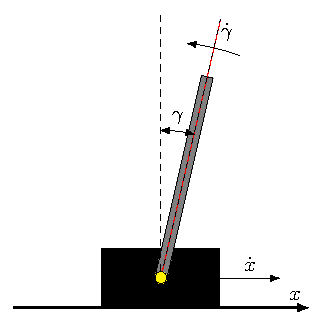
\includegraphics[width = 0.5\textwidth]{plots/cartpole/cartpole_env}
\caption{Cart-Pole environment representation.}
\label{fig:cartpole-env}
\end{figure}
The goal is to keep the pole in the vertical position ($\gamma=0$) as long as possible. The episode ends when the pole reaches a certain angle ($|\gamma| > \bar{\gamma}$) or after a predefined number of steps. We want to encourage smaller forces, to this end we use the following reward function:
$$
R(s,a,s') = 10 - \frac{\omega^2}{20} - 20 \cdot (1 - \cos(\gamma)) .
$$
The first part is a fixed reward for each for each timestep the pole is up and the pole angle is inside the range $[-\bar{\gamma}, +\bar{\gamma}]$. The second part is a penalty proportional to the force. The third part is a penalty proportional the pole angle, it is 0 when the pole is in the vertical position. Ideally the agent should learn to balance the pole with the smaller force possible, keeping it fixed in the vertical position. \newline
\subsection{Results}
We test the performance of REMPS both in the case of an exact model and in the case of an approximated (fitted) model. 
In \cref{fig:cartpole-exp} we show the performance of our algorithm starting from a fixed value of the model parameter, $\omega_0=8$.
\begin{figure}[tb]
\centering
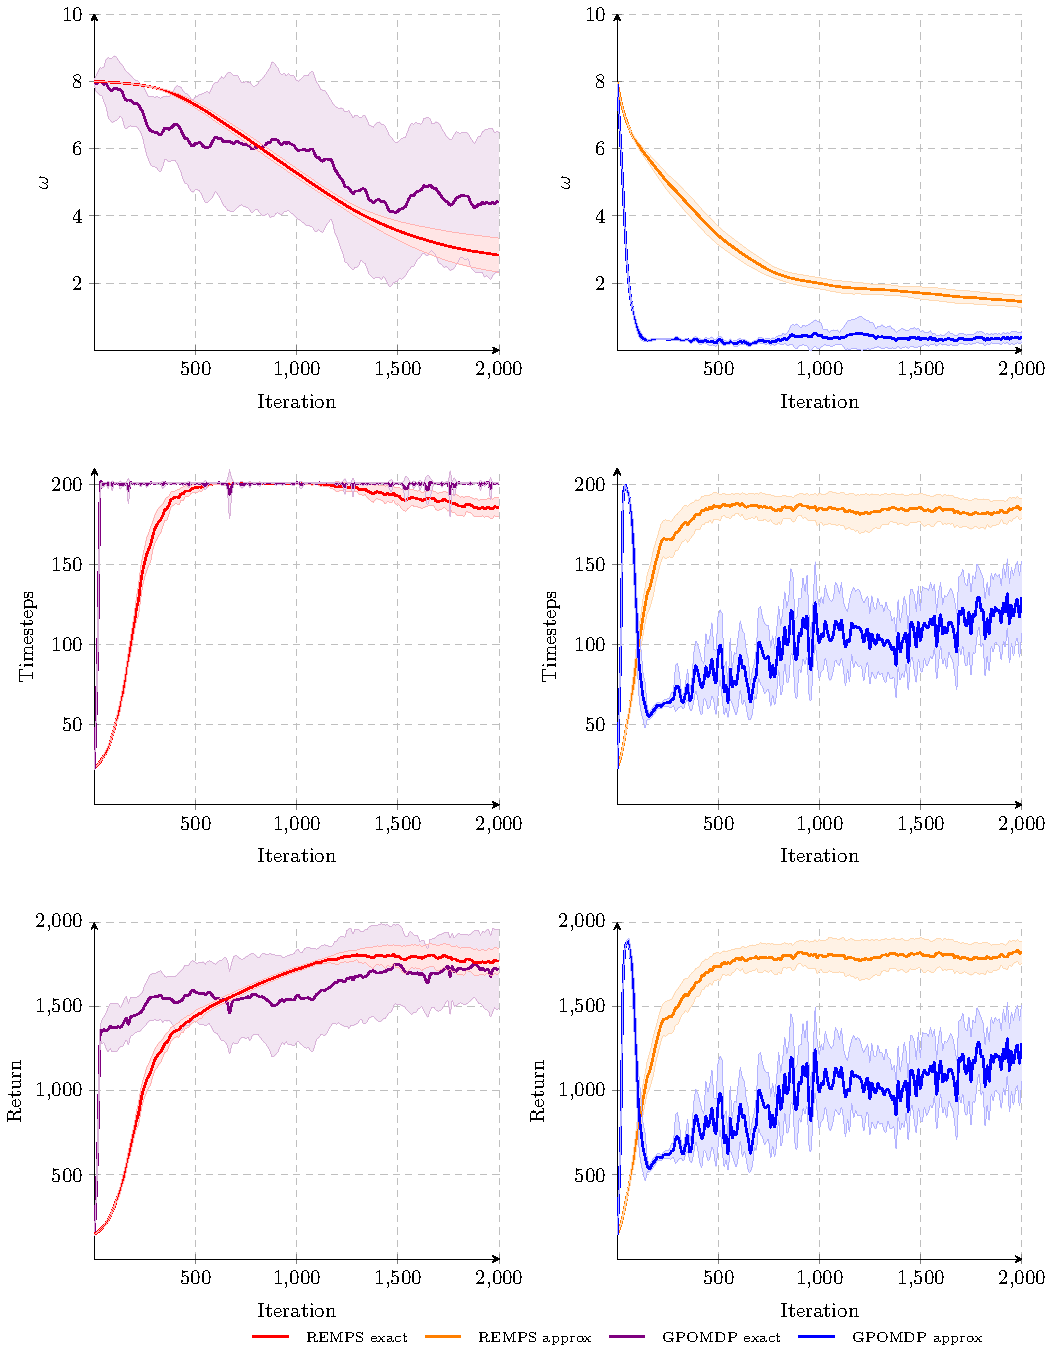
\includegraphics[width = \textwidth]{plots/cartpole/plot_cartpole_experiment}
\caption{Cartpole experiment. Left: results of REMPS and GPOMDP using the exact model. Right: results of REMPS and GPOMDP using the approximated model. Top: model parameter $\omega$. Middle: average timesteps per episode. Bottom: Average return. The shaded area represents the $95\%$ confidence interval over twenty runs of the algorithm.}
\label{fig:cartpole-exp}
\end{figure}
In the exact case, \cref{fig:cartpole-exp} (left), it is possible to see that the model parameter has a decreasing trend in the first iterations, then it converges to a minimum. The timesteps increase and then reach a maximum. The return increases since the agent is less penalized by the force term (since the model parameter is becoming smaller) and it is learning to balance the pole.
In the approximated case, \cref{fig:cartpole-exp} (right),  the cart-pole model is learned by a neural network (NN). The inputs of the NN are the state $s_t$, the action $a_t$ and the model parameter $\omega$. The output neurons represents the mean and the variance of a Gaussian distribution over the state space representing the probability of landing in a given state.
We collect data with a fixed random policy before training. We fitt the dynamic model by maximizing the log-likelihood, obtaining a neural network predicting $P(s' | s, a, \omega)$.
The model learns the effect of the model parameters on the dynamic.
As baseline we use the G(PO)MDP algorithm over the model and policy parameters. Both in the exact version and in the approximated one, REMPS shows a more stable behaviour with respect to G(PO)MDP. In the exact case the two algorithms are comparable, the improvement of REMPS are slower but at the end it outperforms G(PO)MDP with precise selection of the model parameter. \newline
In the approximated case (using the same approximation of the model) REMPS performs better, it is very stable compared to G(PO)MDP. \newline

\begin{table}[!tb]
\centering
\begin{tabular}{ c c}
  \toprule			
  Parameter & Value \\
  \midrule
  Num of samples & $10^5$ \\
  Dual Regularization & 0 \\
  Policy Regularization & 0 \\
  $\epsilon$ & $10^{-3}$ \\
  Policy & Linear with softmax \\
  $\omega_0$ & 8 \\
\bottomrule
\end{tabular}
\caption{Hyper-parameters used in the exact cartpole experiment.} \label{tab:cartpole-hyperparameters-exact}

\vspace*{1 cm}

\begin{tabular}{ c c }
  \toprule			
  Parameter & Value \\
  \midrule
  Num of samples & $5 \cdot 10^4$ \\
  Dual Regularization & $10^{-4}$ \\
  Policy Regularization & $0$ \\
  $\epsilon$ & $10^{-3}$ \\
  Policy & Linear with softmax \\
  $\omega_0$ & 8 \\
\bottomrule
\end{tabular}
\caption{Hyper-parameters used in the approximated cartpole experiment.} \label{tab:cartpole-hyperparameters-approx}

\end{table}

%\begin{table}[!t]
%\centering
%\begin{tabular}{ c c }
%  \toprule			
%  Parameter & Value \\
%  \midrule
%  Num of samples & $5 \cdot 10^4$ \\
%  Dual Regularization & $10^{-4}$ \\
%  Policy Regularization & $0$ \\
%  $\epsilon$ & $10^{-3}$ \\
%  Policy & Linear with softmax \\
%  $\omega_0$ & 8 \\
%\bottomrule
%\end{tabular}
%\caption{Hyper-parameters used in the approximated cartpole experiment.} \label{tab:cartpole-hyperparameters-approx}
%\end{table}


%\paragraph{Random Initialization} In \cref{fig:cartpole-random-init} we compare the approximated versions of REMPS and GPOMDP on the cart-pole experiment with random initialization of the model parameter. For a wide range of the initial model parameter REMPS converges to the optimal parameter. GPOMDP shows an unstable, oscillating behaviour.
%
%
%\begin{figure}[!tb]
%\centering
%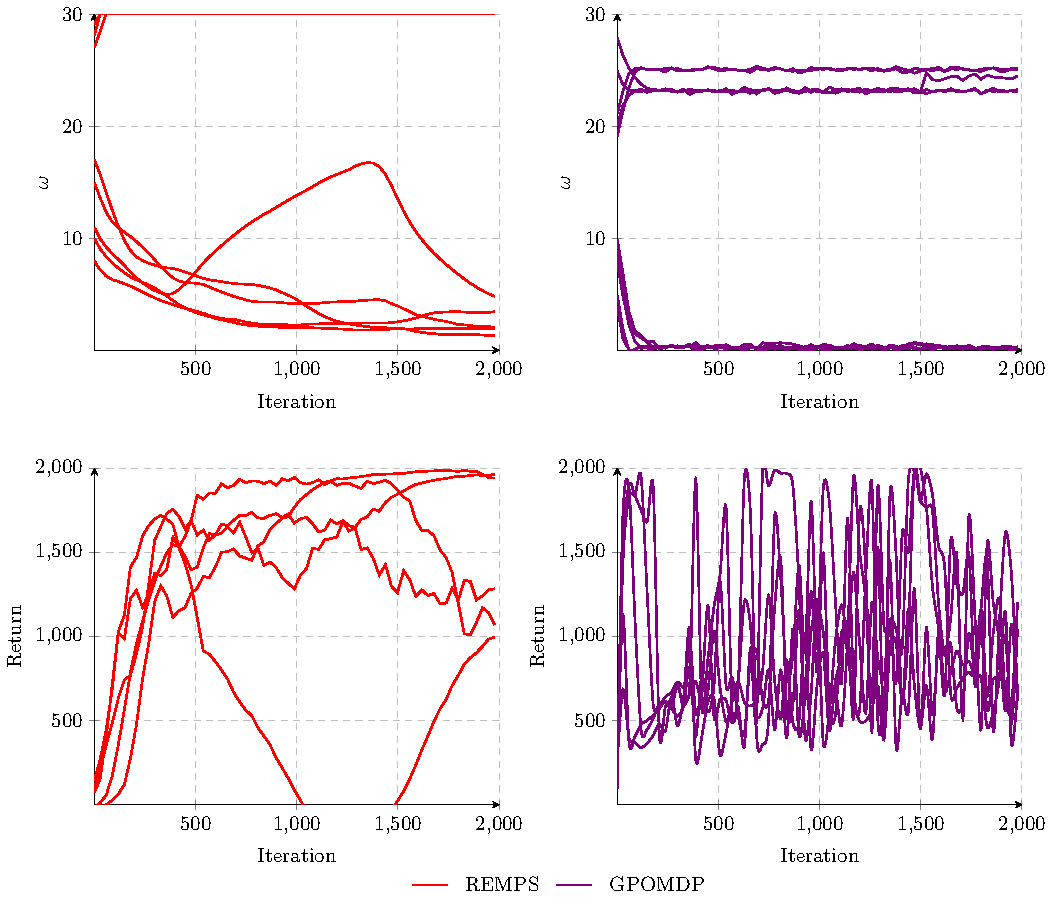
\includegraphics[width = \textwidth]{plots/cartpole/plot-random-init}
%\caption{Cartpole experiment with random initialization of the model parameter. Left: REMPS, right: GPOMDP.}
%\label{fig:cartpole-random-init}
%\end{figure}

\clearpage

\section{Autonomous Driving and Configuration with TORCS}\label{sec:torcs}
The Open Racing Car Simulator \citep{TORCS}, TORCS, is a car racing simulation, which allows to simulate driving races. It is a complete 3D racing simulator offering a complete set of sensors and controls. TORCS has been used as RL environments in \citep{torcs-1, torcs-2, torcs-3, torcs-4} and many others. \newline
We modified the source code of TORCS adding the possibility to configure the car parameters following the "Car Setup Competition".\footnote{https://sourceforge.net/projects/cig} 
The goal of this experiment is to show the benefits of the environment configuration in the context of autonomous driving. 
\subsection{Environment Description}
The state space of the TORCS environment is composed by $29$ dimensions, $\mathcal{S} \subseteq \mathbb{R}^{29}$. The action space is composed by 2 dimensions, $\mathcal{A} \subseteq \mathbb{R}^2$. The first dimension of the action space is the acceleration/brake action, while the second dimension is the steering angle. The configuration space is very large, so we considered only a subset in our experiments.
All configuration parameters are normalized in the range $[0,1]$.
The state space space is summarized in \cref{tab:torcs-state} and the configuration parameters in \cref{tab:torcs-conf}. 
\begin{table}[tb]
\centering
\begin{tabular}{ c | l }
  \toprule			
  Parameter & Description \\
  \midrule
  angle & Angle between the car direction \\
  &  and the direction of the track axis. \\
  rpm & Number of rotation per minute of the car engine. \\
  speedX & Speed of the car along the longitudinal axis of the car. \\
  speedY & Speed of the car along the transverse axis of the car. \\
  speedZ & Speed of the car along the Z axis of the car.\\
  track & Vector of 19 range finder sensors: each sensors returns the \\
  & distance between the track edge and the car within \\
  & a range of 200 meters. \\
  trackPos & Distance between the car and the track axis. \\
  wheelSpinVel & Vector of 4 sensors representing the rotation speed of wheels. \\
\bottomrule
\end{tabular}
\caption{State space of the TORCS experiment.} \label{tab:torcs-state}
\end{table}
\begin{table}[tb]
\centering
\begin{tabular}{ c | l }
  \toprule			
  Parameter & Description \\
  \midrule
  Rear Wing & Angle of the rear wing. \\
  Front Wing & Angle of the front wing. \\
 Front-Rear Brake Repartion & Repartition of the brake between the front and rear. \\
   Front Anti-Roll Bar & Front Spring. \\
  Rear Anti-Roll Bar & Rear Spring.\\
  Front Left-Right Brake & Brake disk diameter of the front wheels.\\
  Rear Left-Right Brake & Brake disk diameter of the rear wheels. \\
\bottomrule
\end{tabular}
\caption{Configuration space of the TORCS experiment.} \label{tab:torcs-conf}
\end{table}
We defined the reward function in the following way:
\begin{equation}
	R(s,a,s') = \text{speedX}' \cdot  \cos ( \text{angle}' ),
\end{equation}
where $\text{speedX}'$ is the velocity on the longitudinal direction of the car in state $s'$ and $\text{angle}'$ is the angle between the car direction and the direction of the track axis.  We give a penalty of $1000$ if the agent runs backward, if it goes out of track or if the progress in the race is too low. The rationale behind this reward is to encourage the agent to go at high speed and to stay centered with respect to the track. \newline
The policy we used in our experiments is a Gaussian Policy parameterized by a fully connected neural network:
\begin{equation}
	\pi(a|s) = \mathcal{N}(\boldsymbol{\phi_m}(s), \boldsymbol{\phi_v}),
\end{equation}
where the mean $\boldsymbol{\phi_m}(s)$ is a non-linear function of the current state $s$ and the variance $\boldsymbol{\phi_v}$ it is independent from the current state. \newline
In the projection phase of REMPS we can only perform a disjoint projection of the policy and model (see \cref{sec:disjproj}) since the state and action spaces are continuous.
\subsection{Results}
In the first phase of our experiments we run a random policy in order to collect the dataset for model fitting. We fitted the model with a neural network using a predefined number of iterations as in \cref{sec:cartpole}. During the actual training phase we used the model network to approximate the system dynamics and we optimized the policy and the environment configuration.
A comparison between the results obtained learning only the policy (REPS) and the results obtained learning the policy and the environment configuration (REMPS) are given in \cref{fig:torcs}. Configuring the environment yields a performance boosting even in an environment with complex dynamic and even starting with a random policy, where the effect of the configuration is limited. We highlight the fact that we learn the model once using a fixed, random policy, while we could alternate model-policy optimization and model fitting for a more precise estimation. 


\begin{figure}[!tb]
\centering
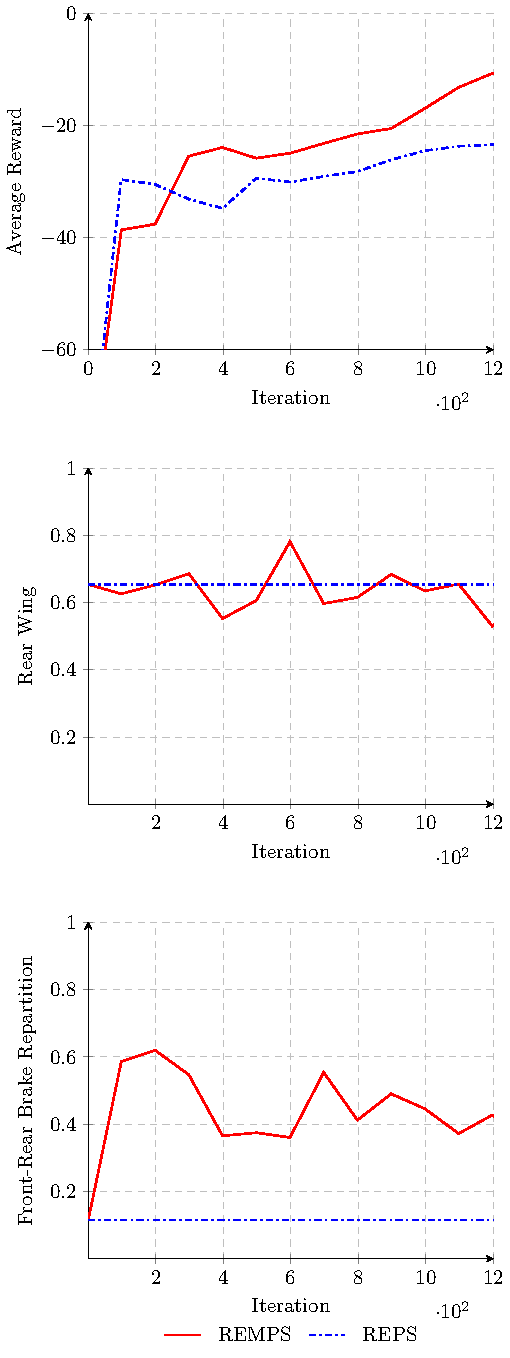
\includegraphics[width = 0.6\textwidth]{plots/torcs/plot_torcs}
\caption{TORCS experiment. Comparison between policy learning and policy-configuration learning. Learning the configuration yields a performance improvement. Top: Average reward. Middle: Rear wing angle. Bottom: Front-Rear Brake repartition.}
\label{fig:torcs}
\end{figure}